\section{Common Geometry and Structural Reductions}
\label{sec:structure-common}
\label{sec:structural-reductions}

We prove the structural facts used by all three mechanisms. The coordinate
calculations are in Appendix~\ref{app:structural-shared-local-signed-center}.

\subsection{Open and closed formulations}

\begin{lemma}[Compact covering margin]
\label{lem:compact-cover-margin}
If a nonempty compact set $K$ is covered by finitely many open unit equilateral
triangles $U_\nu$, then moving every side line inward by the same sufficiently
small positive distance gives a cover by closed equilateral triangles of
side less than one. In particular, $K\subset U$ implies $\Lambda(K)<1$,
with $\Lambda$ defined in \eqref{eq:enclosure-definition}.
\end{lemma}
\begin{proof}
The continuous function
$m(x)=\max_\nu\operatorname{dist}(x,\mathbb R^2\setminus U_\nu)$
has positive minimum $\eta$ on $K$. Move every side line inward by
$0<\rho<\min\{\eta,\sqrt3/6\}$. The resulting closed triangles have
side $1-2\sqrt3\rho$, and each $x\in K$ remains in a triangle realizing
$m(x)\ge\eta>\rho$. Conversely, if $\Lambda(K)<1$, choose a closed
enclosure of side below one and enlarge it about its incenter to side one.
The smaller closed triangle lies in the interior of the enlarged triangle.
\end{proof}

\begin{proposition}[Compactness and scaling equivalence]
\label{prop:open-closed-scaled}
The following assertions are equivalent.
\begin{enumerate}
 \item $H$ is covered by seven open equilateral triangles of side $1$.
 \item For some $\varepsilon>0$, $H$ is covered by seven closed equilateral
 triangles of side $1-\varepsilon$.
 \item For some $L>1$, $H_L:=LH$ is covered by seven closed equilateral
 triangles of side $1$.
\end{enumerate}
\end{proposition}

\begin{proof}
Apply \zcref{lem:compact-cover-margin} to obtain (1)$\Rightarrow$(2).
Enlarging the smaller closed triangles about their incenters gives
(2)$\Rightarrow$(1); dilation by $(1-\varepsilon)^{-1}$ identifies
(2) and (3).
\end{proof}

\begin{lemma}[Distinct triangles]
\label{lem:distinct-roles}
The seven triangles can be labelled so that
\[
 O\in U_C,\qquad V_i\in U_i\quad(0\le i\le5),
\]
and these seven triangles are distinct.  Consequently
\[
 O\in\interior(T_C),\qquad V_i\in\interior(T_i).
\]
\end{lemma}

\begin{proof}
The seven points $O,V_0,\ldots,V_5$ are pairwise at distance at least $1$,
whereas two points of an open unit equilateral triangle are at distance
strictly less than its diameter $1$.  Selecting a covering triangle for each
point therefore gives a bijection.
\end{proof}

\subsection{C triangle and V triangle classifications}

Set
\[
 N_E(T_C):=
 \left\lvert\left\{i\in\mathbb Z/6\mathbb Z:
 \Haus(T_C\cap e_{i,i+1})>0\right\}\right\rvert.
\]
Proposition~\ref{prop:ce-classification} gives $N_E(T_C)\in\{0,1,2\}$;
we call these types $\CEzero,\CEone,\CEtwo$, respectively.

\begin{figure}[H]
\centering
\begin{minipage}[t]{.32\textwidth}
\vspace{0pt}\centering
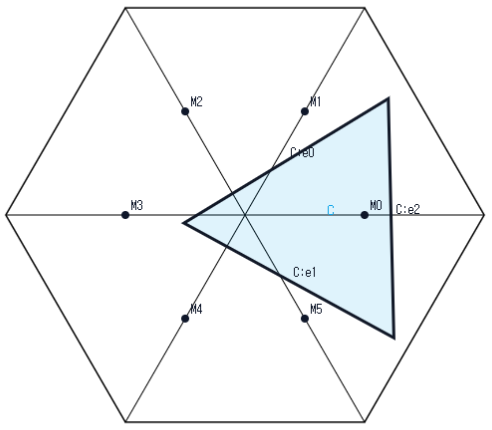
\includegraphics[width=\linewidth,height=.20\textheight,keepaspectratio]
  {figures/role_examples/center_role_ce0_example.png}
\par\smallskip
\footnotesize (a) $\CEzero$
\end{minipage}\hfill
\begin{minipage}[t]{.32\textwidth}
\vspace{0pt}\centering
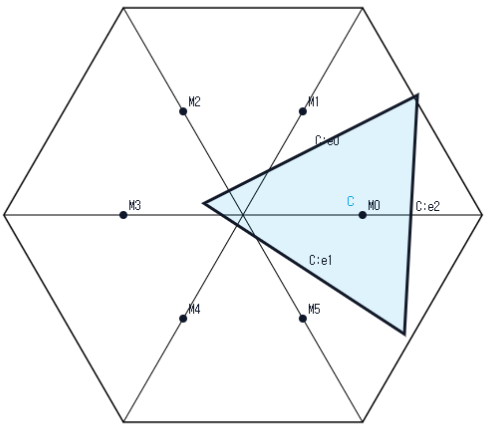
\includegraphics[width=\linewidth,height=.20\textheight,keepaspectratio]
  {figures/role_examples/center_role_ce1_example.png}
\par\smallskip
\footnotesize (b) $\CEone$
\end{minipage}\hfill
\begin{minipage}[t]{.32\textwidth}
\vspace{0pt}\centering
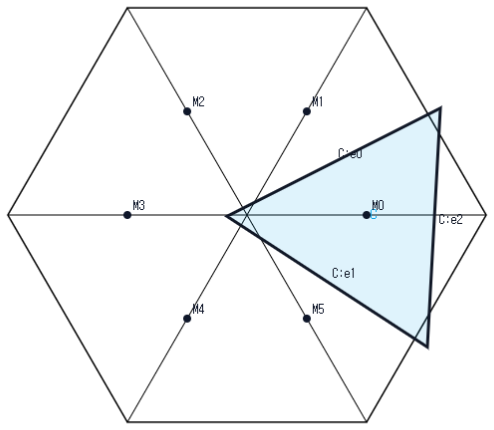
\includegraphics[width=\linewidth,height=.20\textheight,keepaspectratio]
  {figures/role_examples/center_role_ce2_example.png}
\par\smallskip
\footnotesize (c) $\CEtwo$
\end{minipage}
\caption{Examples of the three C triangle classes.  From left to right, the
C triangle has positive-length trace on zero, one, and two edges of
$\partial H$; point contacts do not count.  The panels illustrate the classification.}
\label{fig:center-role-examples}
\end{figure}

Point contacts have zero trace length, so they do not create an additional
positive boundary trace in the definition of $N_E(T_C)$.

\begin{proposition}[Exhaustive center types]
\label{prop:ce-classification}
The closed C triangle $T_C$ has exactly one of the types
$\CEzero,\CEone,\CEtwo$;
equivalently,
\[
 N_E(T_C)\le2.
\]
\end{proposition}

\begin{proof}
If $N_E(T_C)\ge3$, two of the traced edges are nonadjacent in the boundary
six-cycle.  Choose a relative-interior point from each positive-length trace.
By \zcref{lem:app-center-edge-separation}, those points are more than unit
distance apart, so a unit equilateral triangle cannot contain both.
\end{proof}

For the V triangle $T_i$, let $o(T_i)$ be the number of its triangle vertices
outside $H$ and put
\[
 n(T_i)=\left\lvert\left\{j\in\{i-1,i+1\}:
 \Haus(T_i\cap r_j)>0\right\}\right\rvert,
\]
with indices modulo $6$.  The raw pair $(3,0)$ says that all three vertices of
$T_i$ lie outside $H$; it does not say that $T_i$ is disjoint from $H$, since
$V_i\in\interior(T_i)\cap H$.

\begin{lemma}[Local wedge]
\label{lem:local-wedge}
Every original V triangle has $1\le o(T_i)\le3$.  If
$\Haus(T_i\cap r_j)>0$ for some $j\in\{i-1,i+1\}$, at least one vertex of
$T_i$ belongs to $H$; if both adjacent radial traces have positive length,
at least two vertices belong to $H$.
\end{lemma}

\begin{proof}
This is the wedge-incidence calculation in
\zcref{lem:app-local-wedge-calculation}.  The incidence statement concerns the closures; openness is used separately
when forcing points.
\end{proof}

Raw roles with $(o(T_i),n(T_i))=(3,0)$ admit an exact-trace normalization.

\readerheading{Why normalize before measuring reaches?}
The raw case with all three triangle vertices outside $H$ is an incidence
artifact: a translation can leave both its open and closed traces in $H$
unchanged. The next normalization removes that extra case before any actual
reach is defined. It neither enlarges the covered part of $H$ nor changes
which boundary points are covered. This differs from the trace majorant
introduced later, which is not a new open covering triangle.

\begin{proposition}[Exact-trace normalization of raw $(3,0)$ roles]
\label{prop:vd0-exact-trace-normalization}
Let $U$ be an original open V triangle at $V_i$, put $T=\overline U$, and
suppose $(o(T),n(T))=(3,0)$.  There is a same-orientation translate
$\widehat U$, with closure $\widehat T$, such that
\begin{equation}
 V_i\in\widehat U,\qquad (o(\widehat T),n(\widehat T))=(2,0),
 \label{eq:o3-normalized-type}
\end{equation}
and
\begin{equation}
 T\cap H=\widehat T\cap H,\qquad
 U\cap H=\widehat U\cap H.
 \label{eq:o3-exact-traces}
\end{equation}
In particular, all three actual maximal reaches, and whether the two boundary reaches
have sum greater than one, are unchanged.
\end{proposition}

\begin{proof}
The two-orientation affine calculation and the trace-preserving translation
are given in \zcref{lem:app-vd0-trace-normalization-calculation}.
\end{proof}

We apply this translation simultaneously and reuse $U_i,T_i$ for the
normalized triangles.

The normalized exhaustive types used below are
\[
\begin{array}{c|c}
(o(T_i),n(T_i))&\text{established type}\\ \hline
(1,0)&\Vdzero\\
(2,0)&\Vdzero\\
(1,1)&\Vdone\\
(1,2)&\Vdtwo\\
(2,1)&\Tlike.
\end{array}
\]

\begin{proposition}[Exhaustive normalized vertex types]
\label{prop:vertex-classification}
Every normalized V triangle has exactly one of the four types
$\Vdzero,\Vdone,\Vdtwo,\Tlike$ in the displayed type dictionary.
\end{proposition}

\begin{proof}
Lemma~\ref{lem:local-wedge} gives $o\le2$ when $n\ge1$ and $o\le1$ when
$n=2$, while $o\ge1$.  Proposition
\ref{prop:vd0-exact-trace-normalization} replaces the only additional raw
pair, $(3,0)$, by $(2,0)$.
\end{proof}

The next construction is a trace majorant, not a new open covering triangle.

\begin{proposition}[T3-like closed-trace domination]
\label{prop:t3-translation}
Let $T$ be the closure of an original $\Tlike$ V triangle at $V_i$.  There is
a same-orientation translate $\widehat T$ such that
\[
 V_i\in\operatorname{relint}(\text{a side of }\widehat T),
 \qquad T\cap H\subsetneq\widehat T\cap H,
\]
and $(o(\widehat T),n(\widehat T))=(2,1)$, while
\[
 \interior(T)\cap(H\setminus\{V_i\})\subseteq\interior(\widehat T).
\]
Since $V_i$ becomes a boundary point, $\widehat T$ is only a closed-trace
majorant.
\end{proposition}

\begin{proof}
See the two-orientation feasibility calculation in
\zcref{lem:app-t3-translation-calculation}.
\end{proof}

\subsection{Initial reaches and boundary gaps}

The actual maximal reaches are
\[
 A_i:=\max\{x\in[0,1]:V_i+x(V_{i-1}-V_i)\in T_i\},
\]
\[
 B_i:=\max\{x\in[0,1]:V_i+x(V_{i+1}-V_i)\in T_i\},
\]
\[
 C_i:=\max\{x\in[0,1]:V_i+x(O-V_i)\in T_i\}.
\]
The same numbers are the suprema of the corresponding reaches in the open
triangle $U_i$. The V triangle $T_i$ is \emph{supercritical} when
$A_i+B_i>1$, and \emph{nonsupercritical} when $A_i+B_i\le1$. Put
\begin{equation}
 N_+:=\left\lvert\left\{i\in\mathbb Z/6\mathbb Z:
 A_i+B_i>1\right\}\right\rvert.
 \label{eq:N-plus-definition}
\end{equation}
Lowercase reaches are used only after a selection satisfying
\[
 0\le a_i\le A_i,\qquad 0\le b_i\le B_i,\qquad 0\le c_i\le C_i.
\]
They never define $N_+$.

\begin{lemma}[Initial reach segments]
\label{lem:reach-initial-segments}
On the three segments from $V_i$ toward $V_{i-1},V_{i+1},O$, the closed
parameter sets are respectively
\[
 [0,A_i],\qquad[0,B_i],\qquad[0,C_i],
\]
and the open parameter sets are
\[
 [0,A_i),\qquad[0,B_i),\qquad[0,C_i).
\]
Thus the closed maxima equal the corresponding open-triangle suprema.
\end{lemma}

\begin{proof}
The other endpoint of each segment is a distinguished point at distance
one from $V_i$, and is not even in $T_i$: otherwise moving $V_i$
slightly away from it inside $U_i$ would exceed diameter one.
Thus $0<A_i,B_i,C_i<1$. Each intersection with a segment issuing from
$V_i$ is convex.  Closedness of $T_i$, openness of $U_i$, and
$T_i=\overline{U_i}$ give the stated endpoints.
\end{proof}

Parametrize $e_{i,i+1}$ from $V_i$ to $V_{i+1}$ by
\[
 X_i(x):=V_i+x(V_{i+1}-V_i),\qquad 0\le x\le1.
\]
Define the \emph{boundary gap}
\[
 J_i:=e_{i,i+1}\setminus(U_i\cup U_{i+1}),\qquad
 N_{\mathrm{gap}}:=|\{i:J_i\ne\varnothing\}|.
\]
Lemma~\ref{lem:gap-exhaustion} gives
$J_i=X_i([B_i,1-A_{i+1}])$ when $B_i+A_{i+1}\le1$, and $J_i=\varnothing$
otherwise. Equality is a singleton gap, not an overlap.

\begin{lemma}[Exhaustiveness of the gap split]
\label{lem:gap-exhaustion}
One has
\[
 J_i=\begin{cases}
 X_i([B_i,1-A_{i+1}]),&B_i+A_{i+1}\le1,\\
 \varnothing,&B_i+A_{i+1}>1.
 \end{cases}
\]
Every nonempty gap, including a singleton, is missed by all open V triangles.
Under a hypothetical cover it lies in $U_C$ and creates a positive-length
C triangle trace.
Consequently a closed C triangle $T_C$ of type
$\CEzero,\CEone,\CEtwo$ permits respectively at most $0,1,2$ gaps, and
\[
 N_{\mathrm{gap}}=0
 \iff U_0,\ldots,U_5\text{ cover }\partial H.
\]
\end{lemma}

\begin{proof}
By \zcref{lem:reach-initial-segments}, the incident open traces have
parameters $[0,B_i)$ and $(1-A_{i+1},1]$. Their complement is the stated
closed interval.
A nonincident V triangle cannot contain a relative-interior point of the edge:
that point is more than unit distance from its distinguished vertex.  Hence a
gap lies in $U_C$; openness turns even a singleton V-gap into a
positive-length C trace.  Proposition~\ref{prop:ce-classification} gives the
count and the final equivalence.
\end{proof}

\readerheading{Why the threshold is one.}
On a gap-free edge, the open traces overlap, so $B_i+A_{i+1}>1$.
If every edge is gap-free, summing gives
\[
 6<\sum_{i=0}^5(B_i+A_{i+1})=\sum_{i=0}^5(A_i+B_i).
\]
At least one V triangle must therefore be supercritical. A nonempty gap
breaks this cyclic argument: it is precisely where the C triangle takes
over a boundary obligation. Equality $B_i+A_{i+1}=1$ still leaves the
common endpoint uncovered by the two open V triangles; it belongs to the
gap branch, not to the overlap branch.

The distinction between actual and selected reaches is also geometric.
The numbers $A_i,B_i,C_i$ describe a fixed triangle. The later lower bounds
$a_i,b_i,c_i$ prescribe points it must contain and may be reduced when making
a common comparison. Reducing a demand does not change the original
triangle or the count $N_+$.


\begin{lemma}[T3-like V triangles are nonsupercritical]
\label{lem:t3-nonsupercritical}
Every original $\Tlike$ V triangle satisfies
\begin{equation}
 A_i+B_i\le1.
 \label{eq:t3-nonsupercritical}
\end{equation}
Moreover $M_i\notin T_i$. In particular, a T3-like role is not counted
by $N_+$ and cannot supply its own midpoint.
\end{lemma}

\begin{proof}
Both assertions follow from the Type-II calculation in
\zcref{lem:app-t3-translation-calculation}.
\end{proof}

A V role has \emph{positive adjacent-radial support}, or simply
\emph{positive support}, when $n(T_i)>0$. Put
\[
 N_{\mathrm{sp}}:=|\{i:n(T_i)>0\}|.
\]
Positive-support roles are nonsupercritical, so the number of roles that
are supercritical or have positive adjacent-radial support is
$N_++N_{\mathrm{sp}}$. The skeleton budget excludes nonzero-gap covers
with $N_++N_{\mathrm{sp}}\ge3$.

\begin{figure}[H]
\centering
\begin{minipage}[t]{.32\textwidth}
\vspace{0pt}\centering
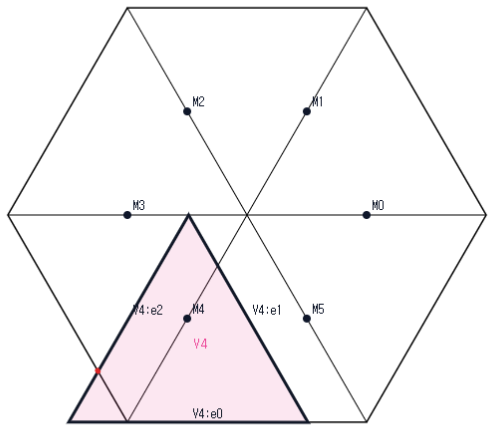
\includegraphics[width=\linewidth,height=.22\textheight,keepaspectratio]
  {figures/role_examples/vertex_role_vd0_axis_aligned_example.png}
\par\smallskip
\footnotesize (a) axis-aligned $\Vdzero$
\end{minipage}\hfill
\begin{minipage}[t]{.32\textwidth}
\vspace{0pt}\centering
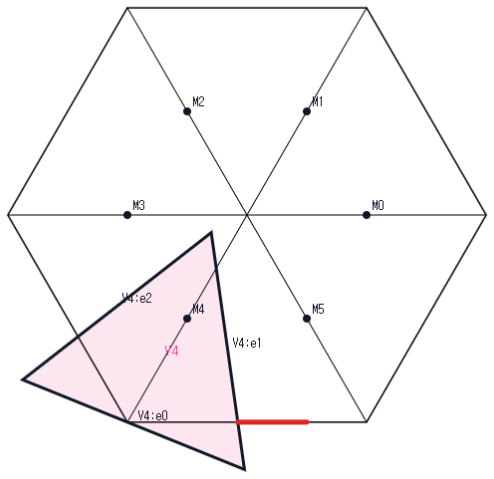
\includegraphics[width=\linewidth,height=.22\textheight,keepaspectratio]
  {figures/role_examples/vertex_role_vd0_nonsupercritical_example.png}
\par\smallskip
\footnotesize (b) nonsupercritical $\Vdzero$
\end{minipage}\hfill
\begin{minipage}[t]{.32\textwidth}
\vspace{0pt}\centering
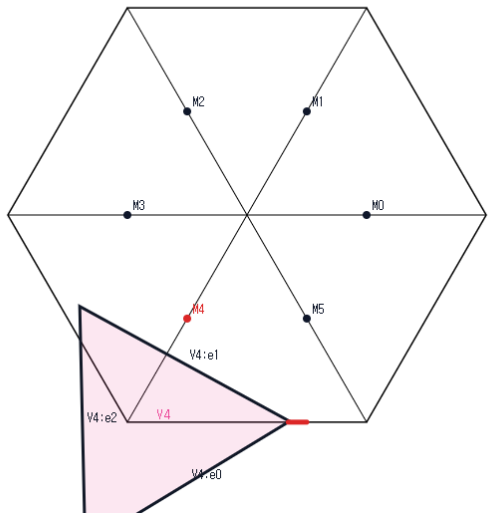
\includegraphics[width=\linewidth,height=.22\textheight,keepaspectratio]
  {figures/role_examples/vertex_role_vd0_supercritical_example.png}
\par\smallskip
\footnotesize (c) supercritical $\Vdzero$
\end{minipage}
\par\medskip
\begin{minipage}[t]{.32\textwidth}
\vspace{0pt}\centering
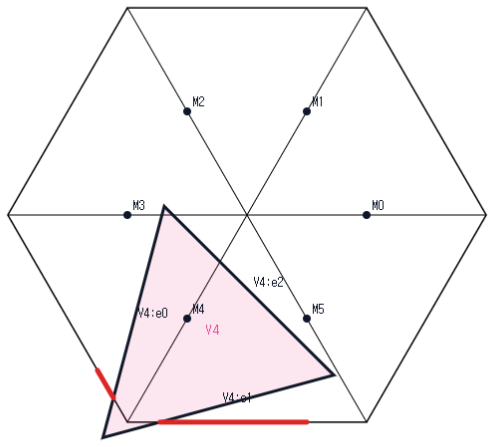
\includegraphics[width=\linewidth,height=.22\textheight,keepaspectratio]
  {figures/role_examples/vertex_role_vd1_example.png}
\par\smallskip
\footnotesize (d) $\Vdone$
\end{minipage}\hfill
\begin{minipage}[t]{.32\textwidth}
\vspace{0pt}\centering
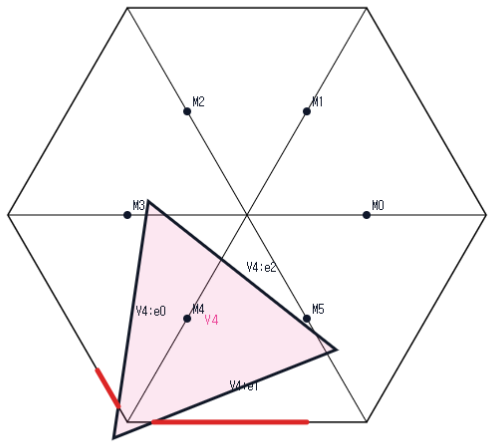
\includegraphics[width=\linewidth,height=.22\textheight,keepaspectratio]
  {figures/role_examples/vertex_role_vd2_example.png}
\par\smallskip
\footnotesize (e) $\Vdtwo$
\end{minipage}\hfill
\begin{minipage}[t]{.32\textwidth}
\vspace{0pt}\centering
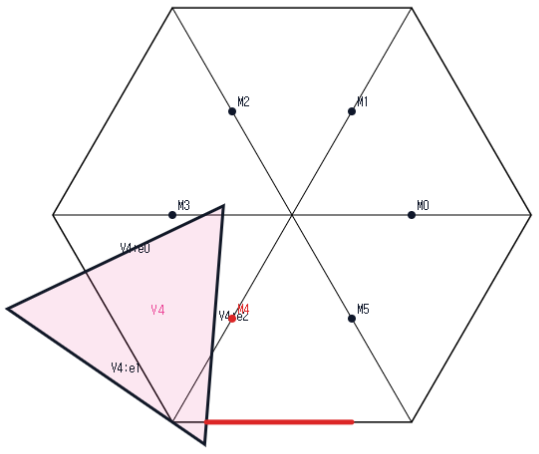
\includegraphics[width=\linewidth,height=.22\textheight,keepaspectratio]
  {figures/role_examples/vertex_role_t3_like_example.png}
\par\smallskip
\footnotesize (f) $\Tlike$
\end{minipage}
\caption{Examples of the normalized V triangle types.  The top row shows an
axis-aligned $\Vdzero$, a nonsupercritical $\Vdzero$ with $A_i+B_i\le1$,
and a supercritical $\Vdzero$ with $A_i+B_i>1$.  The bottom row shows
$\Vdone$, $\Vdtwo$, and $\Tlike$.  The panels illustrate the classification.}
\label{fig:vertex-role-examples}
\end{figure}

\subsection{Strict handoffs and midpoint forcing}

\begin{proposition}[Strict boundary handoffs]
\label{prop:strict-handoffs}
Assume that $U_0,\ldots,U_5$ cover $\partial H$.  There are choices
\[
 \xi_i\in(1-A_{i+1},B_i),\qquad
 a_i:=1-\xi_{i-1},\qquad b_i:=\xi_i,
\]
such that
\[
 0<a_i<A_i,\qquad0<b_i<B_i,\qquad
 a_i^2+a_ib_i+b_i^2<1.
\]
The selected anchors lie in $U_i$.  If exactly one actual V triangle is
supercritical, every strict selection has that same unique selected
supercritical index.  If at least two actual V triangles are supercritical,
some simultaneous strict selection retains at least two.
\end{proposition}

\begin{proof}
The overlap intervals and the cyclic selector are proved in
\zcref{lem:app-strict-handoff-selection}.  Geometrically, each $\xi_i$ lies
in the overlap of two adjacent open edge traces, which makes both associated
reach demands strict.
\end{proof}

\begin{lemma}[Boundary deficit and overlap identities]
\label{lem:boundary-deficit-identities}
For the actual reaches put $s_i=1-A_i-B_i$ and
$\omega_i=B_i+A_{i+1}-1$. Then
\[
 A_{i+1}-A_i=s_i+\omega_i,\qquad
 B_i-B_{i+1}=s_{i+1}+\omega_i.
\]
On a nonsupercritical gap-free path the $A_i$ increase and the $B_i$
decrease strictly. Weak handoffs give the weak version. Around the full
cycle, $\sum_i\omega_i=-\sum_i s_i$.
\end{lemma}
\begin{proof}
Expand the definitions and telescope. Nonsupercriticality gives $s_i\ge0$,
and a gap-free edge has $\omega_i>0$ because its incident traces are open.
A supercritical role has $s_i<0$; propagation through it is not licensed.
\end{proof}

\begin{lemma}[Self-midpoint obstruction]
\label{lem:self-midpoint}
Let $u,v$ be unit vectors meeting at $120^\circ$, and let $a,b\in[0,1]$.
If a closed unit
equilateral triangle contains
\[
 0,\qquad au,\qquad bv,\qquad\frac{u+v}{2},
\]
then $a+b\le1$.  Consequently
\[
 M_i\in T_i\Longrightarrow A_i+B_i\le1.
\]
If the boundary points and midpoint are contained with positive margin, the
conclusion is strict.
\end{lemma}

\begin{proof}
This is the admissible-set corollary
\zcref{lem:app-self-midpoint-caliper}.
\end{proof}

\begin{proposition}[CE1/CE2 exactly-one-midpoint property]
\label{prop:unique-center-midpoint}
If $O\in\interior(T_C)$ and $T_C$ is $\CEone$ or $\CEtwo$, then
\[
 \left|T_C\cap\{M_0,\ldots,M_5\}\right|=1.
\]
This midpoint belongs to $U_C$. Both possible positive boundary traces
are on the two hexagon edges incident to the same vertex.
\end{proposition}

\begin{proof}
Normalize one positive boundary trace.  The signed-center optimization
\zcref{prop:signed-center-normal-form} gives the exact midpoint set
$\{M_0\}$, with radial exit $d_0^C>1/2$ and positive side slacks at
$M_0$. Its boundary traces are confined to $e_{5,0},e_{0,1}$.
Undoing the symmetry proves the assertions.
\end{proof}

The interior hypothesis is essential: $\conv\{O,V_0,V_1\}$ has a boundary
edge overlap and contains both $M_0$ and $M_1$, but $O$ is not interior to it.

\subsection{Exhaustive routing}

When the C triangle has type CE1 or CE2, \zcref{prop:unique-center-midpoint}
shows that it contains exactly one of $M_0,\ldots,M_5$; this is the
\emph{C midpoint}. If it is $M_k$, the role at $V_k$ is called
\emph{center-based}; a supercritical role there is \emph{center-aligned},
and a role at another vertex is \emph{away} or \emph{off-center}.
A V role that contains an adjacent midpoint openly is
called its \emph{supplier} or \emph{rescuer}. A \emph{gap-free
nonsupercritical path} is a consecutive sequence of nonsupercritical V
roles whose shared edges have empty gaps.

We use BC for the selected-gap six-point construction, D for the supported-
midpoint four-point construction, and F for the zero-gap nine-point
construction, all defined in Section~\ref{sec:finite-enclosure}.
N0 denotes \zcref{thm:fixed-nzero}, the assertion that every skeleton
cover has a supercritical V role.

Zero gaps mean that the V triangles cover $\partial H$, and the proof
splits according to $N_+$. With a gap, the C triangle is CE1 or CE2;
N0 and the skeleton budget leave one supercritical role and at most one
positive-support role. Its position relative to the C midpoint determines
the remaining obstruction.

\begin{table}[H]
\centering\small
\setlength{\tabcolsep}{5pt}\renewcommand{\arraystretch}{1.15}
\begin{tabular}{@{}ccp{.34\textwidth}p{.28\textwidth}@{}}
\toprule
$N_{\rm gap}$&$N_+$&Additional condition&Closing mechanism\\
\midrule
$0$&$0$&Arbitrary V types&Strict overlap\\
$0$&$1$&Arbitrary V types&Nine-point F\\
$0$&$\ge2$&Arbitrary V types&Cyclic area loss\\
\midrule
$\ge1$&$0$&Arbitrary V types&N0, through BC\\
$\ge1$&$\ge1$&$N_+\ge2$ or $N_++N_{\rm sp}\ge3$&Skeleton budget\\
$\ge1$&$1$&$N_{\rm sp}\le1$&Midpoint supplier: BC, D, replacement, or Vd2 length\\
\bottomrule
\end{tabular}
\caption{Disjoint routes for the original open cover. Nonzero gaps force
CE1 or CE2; both classes share the same placement reduction. Replacement
preserves the skeleton and ends at N0, without preserving number of gaps.}
\label{tab:routing}
\end{table}

The rows are disjoint and exhaustive: separate zero from nonzero gaps,
then $N_+=0$, and finally the displayed high-count condition.
Lemma~\ref{lem:midpoint-supplier} resolves the last row. BC uses the same
selected-gap witness in CE1 and CE2, with separate candidate calculations.
